\section{Generadores aleatorios}

\subsection{Sistemas de implicaciones aleatorios}

    \textbf{Introducci\'on}

    Cuando se quieren realizar pruebas con un algoritmo, se aconseja utilizar conjuntos generados de forma aleatoria, para que, por ejemplo, 
    en los an\'alisis de tiempo, los resultados no sean influidos por dichos conjuntos. Actualmente, hasta donde se conoce, no existe un 
    generador aleatorio de sistemas de implicaciones en ninguna de las diferentes \'areas, como pueden ser data mining, machine learning, 
    IA, sistemas inteligentes, redes neuronales...

    Por este motivo, se ha decidido realizar una funci\'on que pueda ser usada para este fin y ponerla a disposici\'on de toda la comunidad 
    junto a este paquete.
    \\ 


    \textbf{Descripci\'on}
    
    Esta funci\'on va a generar uno o m\'as sistemas de implicaciones siguiendo una serie de par\'ametros que se pueden elegir a la 
    hora de ejecutar dicha funci\'on.

    Los atributos de las implicaciones van a ser del tipo a0, a1... Comenzando en 0, de forma consecutiva hasta el n\'umero que sea 
    necesario para tener todos los atributos que el usuario quiera. Los par\'ametros de esta funci\'on son:

    \begin{itemize}
        \item \textbf{numAttributes:}

        Aqu\'i se debe especificar cu\'antos atributos diferentes se quiere que tengan las implicaciones que se van a generar. Es un 
        par\'ametro obligatorio para la utilizaci\'on de esta funci\'on. Como se ha comentado anteriormente, los atributos ser\'an de la 
        forma a0, a1, a2... El valor de este par\'ametro debe ser mayor que 0.

        \clearpage

        \item \textbf{numDependencies:}

        Otro par\'ametro obligatorio es el n\'umero de dependencias que se quieren obtener, si se elige obtener m\'as de un archivo 
        con diferentes sistemas de implicaciones, como se ver\'a m\'as adelante, cada uno de dichos ficheros incluir\'a el n\'umero 
        de implicaciones que se le indique aqu\'i. Por supuesto, el valor de este par\'ametro tambi\'en debe ser mayor que 0.

        
        \item \textbf{difference:}

        Este par\'ametro opcional indica la m\'axima diferencia de elementos entre el antecedente y el consecuente. Se puede 
        insertar un n\'umero negativo, lo que indicar\'a que se desea que haya m\'as atributos en el consecuente. Por lo que, si el n\'umero 
        es positivo, el antecedente tendr\'a m\'as atributos.

        En este caso, hay que tener en cuenta que el valor absoluto del n\'umero insertado en este par\'ametro, debe ser menor 
        que el n\'umero total de atributos.

        En caso de no especificar nada, la diferencia de atributos entre antecedente y consecuente ser\'a aleatoria.


        \item \textbf{percentage:}

        Este par\'ametro es bastante parecido al anterior, solo que en este caso, se trata del m\'aximo porcentaje de diferencia entre 
        el antecedente y el consecuente. Al igual que en el anterior, si el porcentaje es negativo, el consecuente ser\'a mayor, y en caso de 
        ser positivo, el antecedente tendr\'a m\'as atributos que el consecuente. Al ser un porcentaje, el valor debe ser menor estricto que 
        100.

        Cabe especificar, que tanto este par\'ametro, como el anterior, se tratan de tama\~nos m\'aximos, es decir, que no todas las implicaciones 
        van a tener la diferencia exacta que se le especifique entre antecedente y consecuente, sino que el n\'umero o porcentaje ser\'a la 
        mayor diferencia que se encontrar\'a en el sistema de implicaciones.


        \item \textbf{maxLeftSize:}

        Con este par\'ametro opcional, se puede especificar el n\'umero de elementos m\'aximo que se quiere que tenga el antecedente, como 
        es de esperar, no debe superar al n\'umero total de atributos.


        \item \textbf{maxRightSize:}

        Junto con el anterior, podemos especificar, en este caso, el n\'umero de elementos m\'aximo del consecuente. Ambos son par\'ametros 
        opcionales, pero si el usuario decide especificar el tama\~no m\'aximo del antecedente, tambi\'en deber\'a hacer lo mismo con el 
        consecuente y viceversa.


        \item \textbf{nameExitFile:}

        Este se trata de un par\'ametro obligatorio, se le debe pasar una cadena de caracteres sin la extensi\'on del archivo, ya que 
        la funci\'on devolver\'a un archivo con extensi\'on .R.


        \item \textbf{numFiles:}

        Otro par\'ametro opcional en el que se puede especificar cu\'antos ficheros se quiere que se generen. Si no se especifica, 
        solo se generar\'a un archivo, en caso contrario, los archivos tendr\'an como nombre el especificado seguido de un guion bajo y un n\'umero 
        para distinguirlos.

        \item \textbf{redundancy:}

        Por \'ultimo, como par\'ametro opcional, se puede elegir si el conjunto de implicaciones que se genere va a tener, o no, redundancias. Si 
        no se especifica este par\'ametro, se aplicar\'a la funci\'on para eliminar redundancias, en caso de que se quiera lo contrario, se 
        deber\'a poner a FALSE.

    \end{itemize}

    Hay que precisar, que algunos de los par\'ametros anteriores son excluyentes. Es decir, si se especifica el par\'ametro \textit{difference}, tanto 
    \textit{percentage}, como \textit{maxLeftSize} y \textit{maxRightSize} deben dejarse nulos. O si se especifica \textit{percentage}, deber\'an quedar vac\'ios \textit{difference} y 
    \textit{maxLeftSize} y \textit{maxRightSize}. 
    En cambio, \textit{maxLeftSize} siempre debe ir acompa\~nado de \textit{maxRightSize} y viceversa, aunque en caso de especificarlos, \textit{difference} y \textit{percentage}, 
    deben estar nulos.
    Los par\'ametros que siempre se le deben pasar a la funci\'on son: \textit{numAttributes}, \textit{numDependencies} y \textit{nameExitFile}.

    Por \'ultimo, hay que especificar que al sistema o sistemas de implicaciones que se obtengan se le habr\'a aplicado 
    la funci\'on de composici\'on, por lo que al realizar esta operaci\'on, si el n\'umero de implicaciones que se quiere obtener es 
    alto, el tiempo que tardar\'a el algoritmo en obtener dicho sistema, tambi\'en ser\'a algo m\'as alto, aumentando dicho tiempo si se quieren 
    eliminar redundancias tambi\'en.
    \\

    \bigskip

    \textbf{C\'odigo}

    \lstinputlisting{r_code/randomGenerators/randomImp.R}
    \bigskip


    \textbf{Ejemplo}

    Como se ha visto anteriormente, este algoritmo se puede utilizar con muchas combinaciones diferentes dependiendo de los par\'ametros 
    que se utilicen. As\'i que, se van a proponer tres ejemplos diferentes de c\'omo usar esta funci\'on, aunque las posibilidades 
    son mucho mayores.

    \bigskip

    \begin{figure}[H]
        \centering
        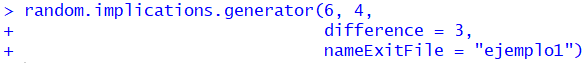
\includegraphics{randomImp1}
        \caption{Ejemplo 1 de sistemas de implicaciones aleatorios}
        \label{fig:randomImp1}
    \end{figure}

    En este primer ejemplo, se va a generar un sistema con cuatro implicaciones, utilizando 6 atributos diferentes, con una diferencia m\'axima 
    de 3 elementos entre el antecedente y el consecuente, siendo mayor el antecedente, como nombre del fichero se utilizar\'a \textit{ejemplo1}. 
    Y como no se especifica el par\'ametro \textit{redundancy}, pues el sistema generado se obtendr\'a con todas las redundancias eliminadas.
    
    En dicho fichero se ha escrito lo siguiente:

    \begin{verbatim}
        a1 a3 a4 a6 -> a5 
        a1 a2 a4 a5 -> a6 
        a3 a6 -> a4 
        a1 a2 a6 -> a3    
    \end{verbatim}


    \begin{figure}[H]
        \centering
        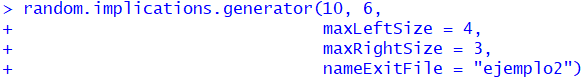
\includegraphics{randomImp2}
        \caption{Ejemplo 2 de sistemas de implicaciones aleatorios}
        \label{fig:randomImp2}
    \end{figure}

    En este segundo ejemplo se han generado con 10 atributos, 6 implicaciones, con un tama\~no m\'aximo de 4 para el antecedente y 3 para el 
    consecuente. El nombre del fichero de salida ser\'a \textit{ejemplo2}.

    \begin{verbatim}
        a1 a10 a6 a7 -> a9 
        a5 -> a4 
        a10 a3 a6 a8 -> a9 
        a8 -> a9 
        a1 a10 a6 -> a7 
        a3 a7 a9 -> a4 
    \end{verbatim}
    Como se puede observar, la salida cumple todos los requisitos que le hemos puesto. En este caso, se observa que solo se han usado 9 de 
    los 10 atributos que se ped\'ian, ya que con la simplificaci\'on del conjunto, se ha llegado a perder el atributo a2.
    \\
    
    \bigskip

    Por \'ultimo, se ejecuta una tercera vez esta funci\'on para comprobar c\'omo es el error que se produce, en este caso, al pasarle vac\'io 
    el nombre del fichero de salida:

    \begin{figure}[H]
        \centering
        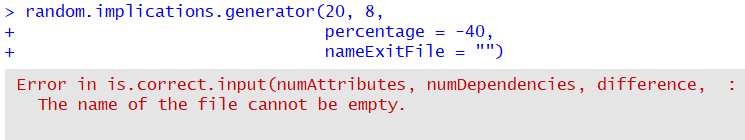
\includegraphics{randomImp3}
        \caption{Ejemplo 3 de sistemas de implicaciones aleatorios}
        \label{fig:randomImp3}
    \end{figure}

    \clearpage


\subsection{Contextos aleatorios}

    \textbf{Introducci\'on}

    En este caso, al igual que en el anterior, hasta donde se sabe, en la comunidad de FCA tampoco existe ning\'un generador aleatorio de 
    contextos, y son bastante necesarios para, como se ha nombrado antes, por ejemplo, realizar pruebas de los diferentes algoritmos, comparativas 
    entre algoritmos, etc.

    As\'i que, se decide realizar un algoritmo de este tipo para a\~nadirlo a este paquete para que toda persona interesada pueda 
    utilizarlo.
    

    \textbf{Descripci\'on}

    Un contexto formal \( (G, M, I) \) consiste en dos conjuntos, G y M, y una relaci\'on binaria \( I \subseteq G x M \). Los elementos 
    de G se llaman objetos, los de M, atributos de \( (G, M, I) \). Si \(g \in G\) y \( m \in M \) est\'an relacionados seg\'un I, se escribir\'a 
    \( (g,m) \in I \) o \( g I m \) y se leer\'a como ``el objeto g tiene el atributo m".\cite{ganter}


    La manera habitual de representar un contexto formal es mediante una tabla, la cual contar\'a con una fila para cada objeto y una columna 
    para cada atributo, con una cruz en la intersecci\'on entre una fila g con una columna m sii el objeto g tiene un atributo m, \( (g,m) \in 
    I \).

    Por ello, la estructura m\'as interesante a la hora de programar un algoritmo para contextos formales en R ser\'a un data.frame.
    \\


    Luego, en este caso, esta funci\'on va a generar un contexto formal siguiendo algunos par\'ametros que se pueden elegir a la 
    hora de ejecutar dicha funci\'on para obtener el contexto. Adem\'as, se generar\'a 
    un archivo csv con el mismo resultado para poder comprobar a posteriori el contexto aleatorio generado.

    Los objetos del contexto se van a representar como obj1, obj2... y los atributos como att1, att2... Ambos comenzando en 1, de forma 
    consecutiva hasta el n\'umero que el usuario indique.
    \\

    Los par\'ametros de esta funci\'on son:

    \begin{itemize}
        \item \textbf{num.obj:}

        Con este par\'ametro obligatorio se indicar\'a el n\'umero de objetos que debe tener el contexto, o lo que es lo mismo, 
        cu\'antas filas tendr\'a el data.frame. Este par\'ametro debe ser mayor que uno, 
        ya que no tendr\'ia sentido crear un contexto sin objetos.


        \item \textbf{num.attr:}

        Este par\'ametro obligatorio indicar\'a cual ser\'a el n\'umero de atributos del contexto, es decir, las columnas que tendr\'a el 
        data.frame. De nuevo, debe ser un n\'umero mayor que uno, ya que tampoco tendr\'ia sentido en este caso crear un contexto sin 
        atributos.

        \item \textbf{sparness:}

        Como par\'ametro opcional, tenemos la dispersi\'on, es decir, el n\'umero de unos. O lo que es lo mismo, la probabilidad 
        de que un objeto tenga un atributo, que a la hora de representarlo, en el cruce de columna y fila, haya un uno.
        Como este par\'ametro se trata de una probabilidad, su valor debe estar entre 0 y 1.

        \item \textbf{namefile:}

        Tambi\'en se puede elegir el nombre que va a tener el fichero de salida. Si no se especifica dicho nombre, por defecto, el 
        csv se llamar\'a \textit{context}.

    \end{itemize}


    Cuando se utilice la funci\'on, esta devolver\'a un data.frame, siendo los nombres de filas los objetos, y los de las columnas 
    los atributos.


    \bigskip

    \textbf{C\'odigo}

    A la hora de optimizar el c\'odigo, si el par\'ametro \textit{sparness} no est\'a vac\'io, se ha decidido generar aleatoriamente el n\'umero de 
    TRUE o FALSE dependiendo de cu\'al de los dos sea menor. Es decir, si el usuario inserta en el par\'ametro \textit{sparness} 0.2, con 4 objetos 
    y 5 atributos, esto querr\'a decir que debe haber cuatro TRUE entre los 20 elementos a generar aleatoriamente. Por lo que en este caso, 
    el n\'umero de TRUE ser\'a menor que el de FALSE, as\'i que se colocar\'an cuatro TRUE aleatoriamente, rellenando las dem\'as posiciones 
    del data.frame a FALSE.

    Como el algoritmo se va a ejecutar de formas diferentes dependiendo de las entradas que elija el usuario, se ha decidido modularizarlo 
    para poder comprenderlo bien. Veamos las diferentes partes:


    Aqu\'i tenemos el algoritmo principal, que ser\'a el que el usuario utilice:

    \lstinputlisting{r_code/randomGenerators/context.R}
    \bigskip

    En el caso de que el usuario no especifique el par\'ametro \textit{sparness}, el contexto se generar\'a totalmente de forma aleatoria:

    \lstinputlisting{r_code/randomGenerators/noSpar.R}
    \bigskip

    Y como se ha especificado anteriormente, dependiendo de cu\'al sea la probabilidad de dispersi\'on elegida por el usuario, se generar\'an 
    los TRUE o los FALSE:

    \lstinputlisting{r_code/randomGenerators/ones.R}
    \clearpage
    \lstinputlisting{r_code/randomGenerators/zeros.R}
    \bigskip

    \textbf{Ejemplo}

    Como primer ejemplo, se va a generar un contexto sin el par\'ametro \textit{sparness}, con 4 objetos y 5 atributos:

    \begin{figure}[H]
        \centering
        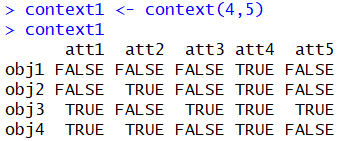
\includegraphics{randomC1}
        \caption{Ejemplo 1 de contextos aleatorios}
        \label{fig:randomC1}
    \end{figure}

    \bigskip
    Y como segundo ejemplo, un contexto con 6 objetos y 8 atributos, con 0.5 de \textit{sparness}:

    \begin{figure}[H]
        \centering
        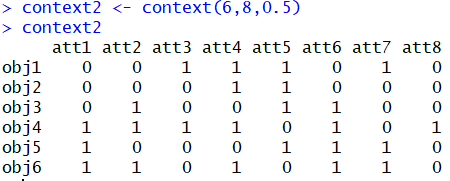
\includegraphics{randomC2}
        \caption{Ejemplo 2 de contextos aleatorios}
        \label{fig:randomC2}
    \end{figure}

    Como podemos observar, el n\'umero de FALSE y TRUE es el mismo, ya que se ha elegido como par\'ametro de \textit{sparness} 0.5.
    

    En ambos casos se genera un fichero csv con dicho contexto con el nombre por defecto \textit{context}, los cuales contienen la misma 
    informaci\'on que los data.frame.

    \newpage
    \thispagestyle{empty}
    \mbox{}
    \newpage